% File: background.tex
% Date: 8.27.2014
% Author: Jared Bold

\chapter{Background}

% Hardware
\section{Hardware}
The hardware platform used is the Xilinx ZC702 Evaluation Board, featuring a Zynq\textsuperscript{\textregistered} XC7Z020 System on a Chip (SoC).

% Operating System
\section{Operating System}
The operating system selected to run on the ZC702 is Linux.  The version used is maintained by Xilinx and is on kernel veresion 3.14.

% Algorithms
\section{Bilinear Interpolation}
Bilinear interpolation (BI) is the process by which an unknown value is interpolated based on a 2 dimensional interpolation process using 4 known values.  In its application in image processing, BI is used to scale images up and down.  Unlike nearest-neighbor interpolation, which relies on only one known value resulting in blocky images, BI has creates smoother images when scaling due to its estimation of intermediate values.

\begin{figure}
  \centering
  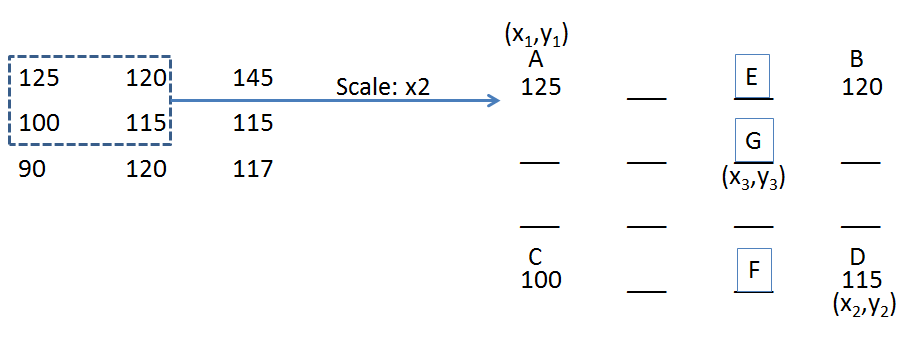
\includegraphics[width=10cm]{./img/bilinear_example.PNG}
  \caption{Bilinear Interpolation of Grayscale Image}
  \label{fig:bilinearExample}
\end{figure}
The process of bilinear interpolation begins by expanding the known pixels to their scaled locations.  This expansion process generates a window of unknown pixels, bounded by four corners of known pixels, as shown in \ref{fig:bilinearExample}.  In order to calculate the the unknown pixel values, three equations must solved.  To generate an final equation for the value, the variables shown in \ref{fig:bilinearExample} will be used.  The first equation is the horizontal interpolation of the value at $E$.
\begin{equation}
  E = \frac{x_3-x_1}{x_2-x_1}B + \frac{x_2-x_3}{x_2-x_1}A
  \label{eqn:E}
\end{equation}
Next, the horizontal interpolation of the value at $F$ is calculated.
\begin{equation}
  F = \frac{x_3-x_1}{x_2-x_1}D + \frac{x_2-x_3}{x_2-x_1}C
  \label{eqn:F}
\end{equation}
Finally, the vertical interpolation of value at $G$ is calculated.
\begin{equation}
  G = \frac{y_3-y_1}{y_2-y_1}F + \frac{y_2-y_3}{y_2-y_1}E
  \label{eqn:G}
\end{equation}

\begin{equation}
  \alpha = x_3 - x_1, 
  \beta = x_2 - x_3, 
  \gamma = y_3 - y_1, 
  \omega = y_2 - y_3
  \label{eqn:rename}
\end{equation}
By substituting \eqref{eqn:E} and \eqref{eqn:F} into \eqref{eqn:G} and allowing variables to be renamed as in \eqref{eqn:rename}, the BI equation for a pixel is determined.
\begin{equation}
  G = \frac{1}{(\omega + \gamma)(\beta + \alpha)}[\gamma(\alpha D + \beta C) + \omega(\alpha B + \beta A)]
  \label{eqn:bilinear}
\end{equation}

By applying \eqref{eqn:bilinear} to every unknown pixel in every window that is generated from the scaling process, an image is enlarged or shrunk with minimal loss of quality.  This technique is easily extended to multiple color channel images such RGB by operating on each colorplane individually and ensuring that pixel offsets are correctly calculated.
